% CodeMixESC architecture for the presentation (16:9). pdflatex architecture_slide.tex
\documentclass[tikz,border=8pt]{standalone}
\usepackage[T1]{fontenc}
\usepackage{helvet}
\renewcommand{\familydefault}{\sfdefault}
\usetikzlibrary{arrows.meta,fit,backgrounds,calc,positioning}
\definecolor{orig}{HTML}{E8EEF7}
\definecolor{origline}{HTML}{4A6A96}
\definecolor{new}{HTML}{FFE3C2}
\definecolor{newline}{HTML}{D9640B}
\definecolor{mod}{HTML}{DCEBFF}
\definecolor{ink}{HTML}{1F2937}
\definecolor{stagebg}{HTML}{F6F8FB}
\begin{document}
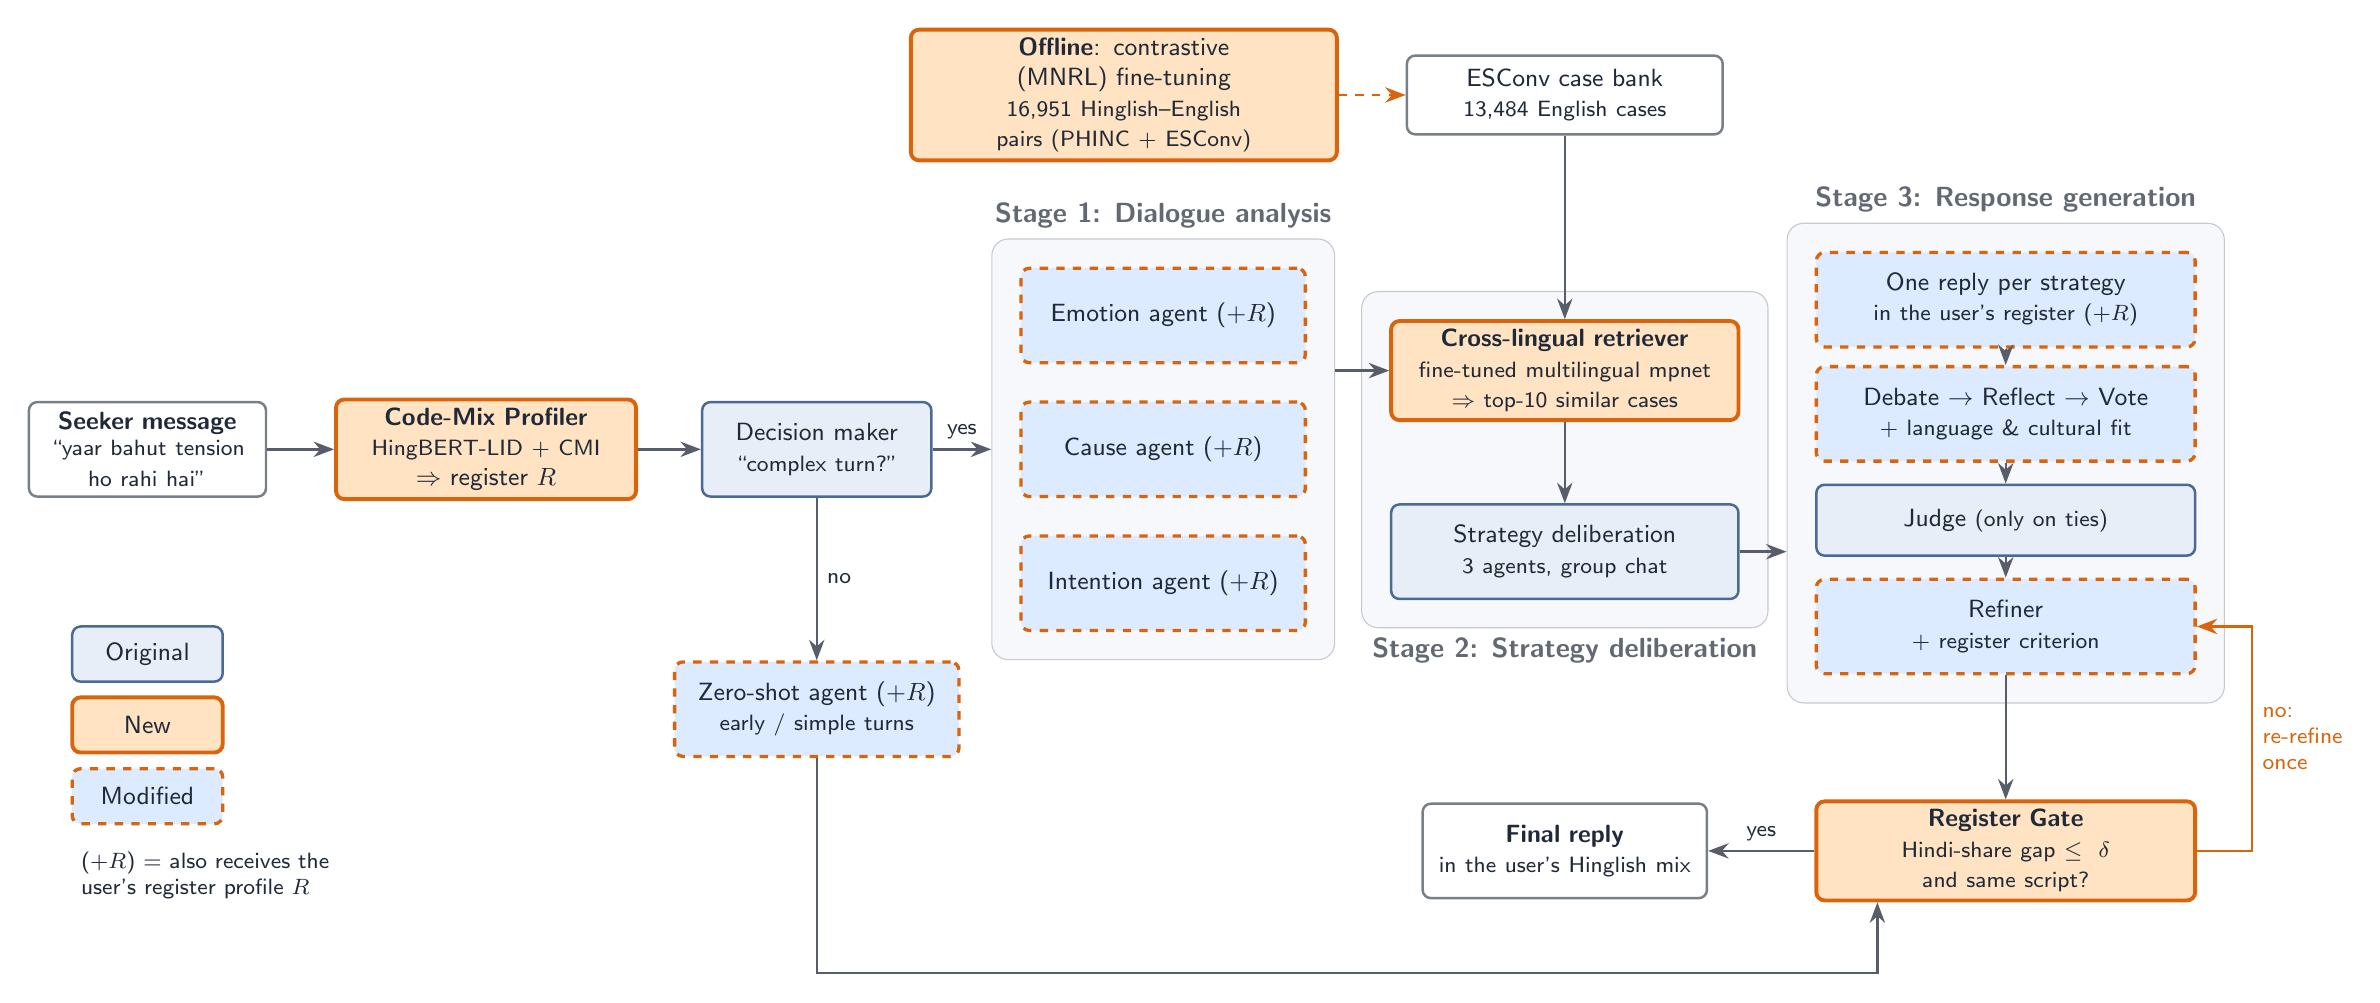
\begin{tikzpicture}[
  font=\sffamily\small, >={Stealth[length=2.6mm]}, line width=0.9pt, ink,
  box/.style={draw=origline, fill=orig, rounded corners=3pt, align=center, minimum height=12mm,
              text width=34mm, inner sep=3pt},
  new/.style={box, draw=newline, fill=new, line width=1.4pt},
  mod/.style={box, draw=newline, fill=mod, dashed, line width=1.2pt},
  io/.style={box, draw=ink!60, fill=white},
  stage/.style={draw=ink!25, fill=stagebg, rounded corners=6pt, inner sep=3.5mm},
  lab/.style={font=\sffamily\bfseries\normalsize, text=ink!70},
  note/.style={font=\sffamily\footnotesize},
  arr/.style={->, draw=ink!75}]
% ---------- input, profiler, decision
\node[io, text width=28mm] (seek) at (0,0) {\textbf{Seeker message}\\{\footnotesize ``yaar bahut tension\\ho rahi hai''}};
\node[new, text width=36mm] (prof) at (4.3,0) {\textbf{Code-Mix Profiler}\\{\footnotesize HingBERT-LID + CMI}\\$\Rightarrow$ register $R$};
\node[box, text width=27mm] (dec) at (8.5,0) {Decision maker\\{\footnotesize ``complex turn?''}};
\node[mod, text width=34mm] (zs) at (8.5,-3.3) {Zero-shot agent (+$R$)\\{\footnotesize early / simple turns}};
% ---------- stage 1
\node[mod] (emo) at (12.9,1.7) {Emotion agent (+$R$)};
\node[mod] (cau) at (12.9,0) {Cause agent (+$R$)};
\node[mod] (int) at (12.9,-1.7) {Intention agent (+$R$)};
% ---------- stage 2
\node[new, text width=42mm] (ret) at (18.0,1.0) {\textbf{Cross-lingual retriever}\\{\footnotesize fine-tuned multilingual mpnet}\\{\footnotesize $\Rightarrow$ top-10 similar cases}};
\node[box, text width=42mm] (del) at (18.0,-1.3) {Strategy deliberation\\{\footnotesize 3 agents, group chat}};
% ---------- offline row
\node[new, text width=52mm, minimum height=10mm] (train) at (12.4,4.5)
      {\textbf{Offline}: contrastive (MNRL) fine-tuning\\{\footnotesize 16,951 Hinglish--English pairs (PHINC + ESConv)}};
\node[io, text width=38mm, minimum height=10mm] (bank) at (18.0,4.5)
      {ESConv case bank\\{\footnotesize 13,484 English cases}};
% ---------- stage 3
\node[mod, text width=46mm] (gen) at (23.6,1.9) {One reply per strategy\\{\footnotesize in the user's register (+$R$)}};
\node[mod, text width=46mm] (deb) at (23.6,0.45) {Debate $\to$ Reflect $\to$ Vote\\{\footnotesize + language \& cultural fit}};
\node[box, text width=46mm, minimum height=9mm] (jud) at (23.6,-0.9) {Judge {\footnotesize (only on ties)}};
\node[mod, text width=46mm] (ref) at (23.6,-2.25) {Refiner\\{\footnotesize + register criterion}};
% ---------- gate and output
\node[new, text width=46mm] (gate) at (23.6,-5.1) {\textbf{Register Gate}\\{\footnotesize Hindi-share gap $\le\delta$ and same script?}};
\node[io, text width=34mm] (out) at (18.0,-5.1) {\textbf{Final reply}\\{\footnotesize in the user's Hinglish mix}};
% ---------- stage frames and labels
\begin{scope}[on background layer]
\node[stage, fit=(emo)(int)] (s1) {};
\node[stage, fit=(ret)(del)] (s2) {};
\node[stage, fit=(gen)(ref)] (s3) {};
\end{scope}
\node[lab, anchor=south] at (s1.north) {Stage 1: Dialogue analysis};
\node[lab, anchor=north] at (s2.south) {Stage 2: Strategy deliberation};
\node[lab, anchor=south] at (s3.north) {Stage 3: Response generation};
% ---------- edges
\draw[arr] (seek) -- (prof);
\draw[arr] (prof) -- (dec);
\draw[arr] (dec) -- node[right, note] {no} (zs);
\draw[arr] (dec.east) -- node[above, note] {yes} (s1.west|-dec.east);
\draw[arr] (s1.east|-ret.west) -- (ret.west);
\draw[arr] (ret) -- (del);
\draw[arr, dashed, newline] (train) -- (bank);
\draw[arr] (bank) -- (ret);
\draw[arr] (del.east) -- (s3.west|-del.east);
\draw[arr] (gen) -- (deb);
\draw[arr] (deb) -- (jud);
\draw[arr] (jud) -- (ref);
\draw[arr] (ref) -- (gate);
\draw[arr] (zs.south) |- ($(gate.south west)+(0.8,-0.9)$) -- ($(gate.south west)+(0.8,0)$);
\draw[arr] (gate) -- node[above, note] {yes} (out);
\draw[arr, newline] (gate.east) -- ++(0.7,0) |- node[pos=0.25, right, note, text=newline, align=left] {no:\\re-refine\\once} (ref.east);
% ---------- legend
\node[box, text width=17mm, minimum height=7mm] (l1) at (0.0,-2.6) {Original};
\node[new, text width=17mm, minimum height=7mm, below=1.6mm of l1] (l2) {New};
\node[mod, text width=17mm, minimum height=7mm, below=1.6mm of l2] (l3) {Modified};
\node[note, anchor=north west, align=left, text width=42mm] at ($(l3.south west)+(0,-0.2)$) {(+$R$) = also receives the\\user's register profile $R$};
\end{tikzpicture}
\end{document}
